\documentclass[a4paper, 12pt]{article}

% Packages
\usepackage{graphicx}
\usepackage[breaklinks]{hyperref}
\usepackage[all]{hypcap}
\usepackage[utf8]{inputenc}
\usepackage[backend=biber]{biblatex}
\usepackage{ifxetex}
\usepackage{breakurl}

% TUB Font
\ifxetex
   % Muli font
   \usepackage{xltxtra}
   \setmainfont{Muli}
\else
   % Arial font
   \usepackage{times}
   \renewcommand{\rmdefault}{\sfdefault}
\fi
\linespread{1.2}

% Settings
\graphicspath{ {images/} }
\addbibresource{bibliography.bib}

% Variables
\newcommand{\thesistitle}{model2regex: Detecting DGAs with Regular Expressions Generated by a Language Model}
\newcommand{\thesisauthor}{Eric Schneider}
\newcommand{\matrno}{365800}
\newcommand{\supervisor}{Alexander \textsc{Warnecke}, Tammo \textsc{Kr\"uger}}
\begin{document}

\begin{titlepage}
	\centering
	
\includegraphics[width=5cm]{tub-logo}\par\vspace{0.5cm}
	{Technische Universität Berlin \par}
	\vspace{2cm}
	{\large \textsc{Exposé}\par}
	\vspace{1cm}
	{\Large\bfseries \thesistitle\par}
	\vspace{2cm}
	%\vfill
	{\large \thesisauthor\par}
	{\large Matr. No. \matrno\par}
	\vspace{2cm}
	
\includegraphics[width=5cm]{mlsec-logo-red2}\par\vspace{0.5cm}
	{Chair of Machine Learning and Security \par}
	{Prof. Dr. Konrad Rieck \par}
	\vfill
	supervised by\par
	\supervisor
	\vfill
	\today\par
\end{titlepage}

\section{Introduction}
%Some intro to the topic: What is it about? What is the specific problem that should be addressed in
%this work?
Domain Generating Algorithms (DGAs) are increasingly used in botnets as part of command and control
(C\&C) communication. This form of malware is used to obfuscate the real server a botnet or other
distributed attacks get their instructions and updates from. By using seeded random generation of
domains, these algorithms create thousands of domains and contact only a small portion of them,
which makes static detection and sinkholing \cite{plohmannComprehensiveMeasurementStudy2016} very
difficult. This strategy gives the attacker a huge advantage, because to protect against it, means
taking control of possible thousands of domains, while the attacker only needs to control a single
short lived domain, during the execution of their attack. A better form of protection would be to
detect, if a network request is towards a potential algorithmically generated domain and block the
communication at the source. DGAs, however, generate domains pseudo-randomly and use different seeds from
either specific dates, twitter trends, hashes or word lists. Therefore static blocklists may not be
able to keep up with blocking the communication at a network level. Deep Learning approaches have
shown great promises and are currently state of the art in detecting Algorithmically-Generated
Domains (AGD). Machine learned models can be used to filter network traffic. Setting them up for a
filter pipeline, however, may not be very simple and act as a black box where it is not entirely
sure what they are filtering.\\ Using algorithms from the field of language processing this thesis
will attempt to learn the structure of different DGA families, using that information to generate
regular expressions (RegEx). Resulting in an ease in implementing filters in existing security
architecture and showing a more human readable result to help understanding the structure of learned
DGAs.

\section{Methodology}
%What methodology will be applied in this work? That is, what is the general strategy to solve the
%problem this work is concerned with?
The main methodology of this thesis will be applied research. Using currently established solutions,
from the field of language processing, I will train a language model that learns the structure of
DGAs and classifies them into their individual DGA families and benign domain names. Once the structure has
been learned the research will focus on the possibility to extract information from the language
model and turn it into a RegEx. If this succeeds then the work will focus on evaluating if the
generated RegEx can compete with the language model itself and solutions of current state of the
art. These approaches will again be iteratively improved upon through research and testing of
strategies for extracting and optimizing the resulting RegEx.
\section{Approach}
%How is the implementation of the strategy approached?
During the prototyping phase, I will use a dataset of the top 1 million domains
\cite{CiscoPopularityList} for benign data and
generate AGDs through reverse engineered DGAs \cite{baderDomainGenerationAlgorithms2024}
as malicious data. During evaluation and
after finalizing the thesis I will try to work with real data from the
DGArchive \cite{DGArchiveFraunhoferFKIE} and real data from
network traffic to test outside of a ''lab setting''.\\
Using these labels, I then learn a recurrent neural network, as shown in Figure \ref{fig:RNNLanguageModel},
more specifically a gated recurrent unit (GRU), a long short-term memory network with gating mechanism.
Instead on a word level, however, this network will work on a character based level to predict the next
character in the sequence to generate the domain.
The language model will turn the possible characters of our domains into word embeddings, then feed
those into the hidden states and then apply a softmax to generate the probability distribution of
the next letter in the sequence.
Additionally I am using the output of the last hidden state to feed the semantic meaning into a feed
forward network to classify the input, as shown in Chapter 9 of the book \textit{Speech and Language
Processing} by Jurafsky and Martin \cite{jurafskyRNNsSequenceClassification2024}.\\ 
After training the language model the next step is to generate regular expressions. This will be
done by using the distribution output by our model after classifying the domain input. The current
idea is to use specific probability thresholds to determine what RegEx atoms will be generated for
each position in the resulting expression.
\begin{figure}[h]
    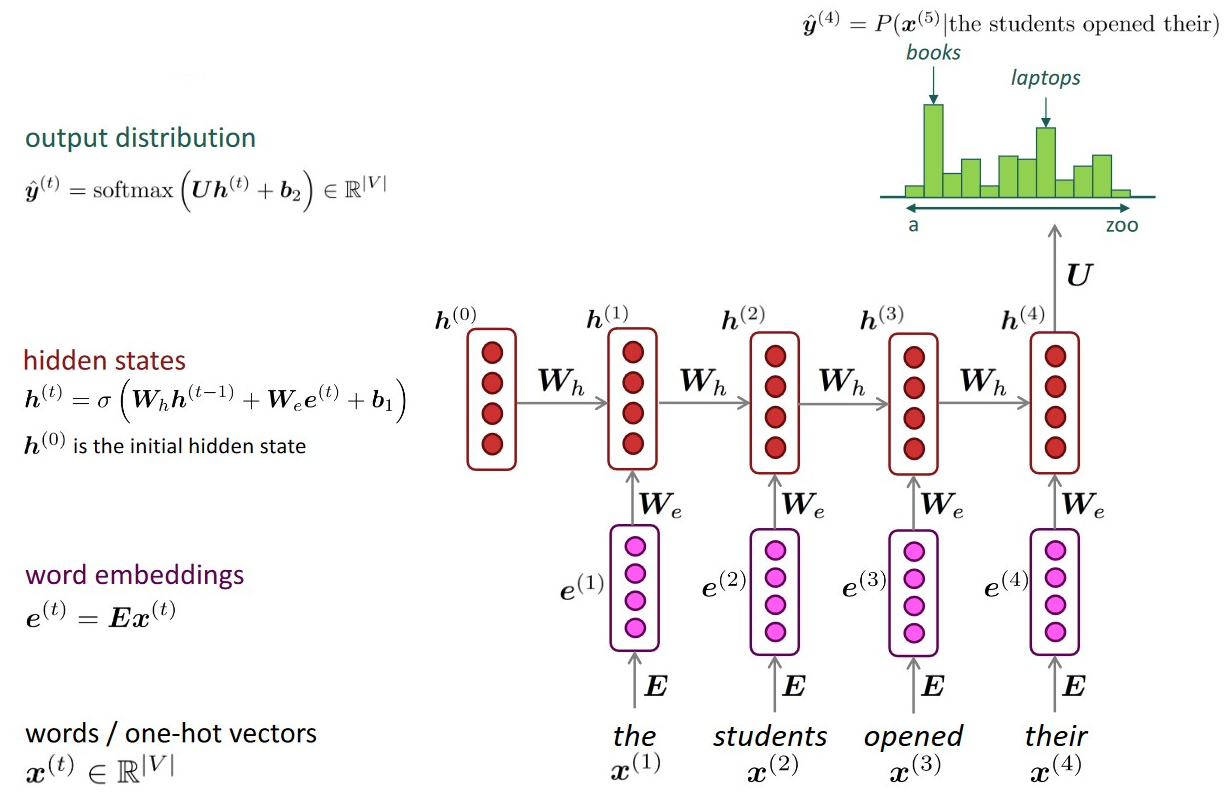
\includegraphics[width=\textwidth]{cs224n-spr2024-lecture05-language-model.png}
    \caption{Example of a RNN Language Model by \cite{manningNaturalLanguageProcessing2024}}
    \label{fig:RNNLanguageModel}
\end{figure}
\section{Evaluation}
%How is the degree of success of the applied method measured?
I will evaluate the result of this thesis by testing how well the generated regular expressions
will capture the learned structures of DGAs.  
The experiment will be set up the following way:\\
The test dataset will be constructed from DGArchive\cite{DGArchiveFraunhoferFKIE} as the source of AGDs and
real network data as the source for benign domains.
Using the dataset I will compare the language model and the RegEx to the NYU model provided by Yu et
al. 
\cite{yuCharacterLevelBased2018}, which was adapted from Zhang et al. \cite{NIPS2015_250cf8b5}. The evaluation will compare Precision, Recall,
$F_1$-score and area under the ROC curve (AUC), between the character based models, my own language
model and the generated regular expression(s). I'll be using a single model from that paper because
all compared solutions are very close in performance therefore I will only need to test with one to
be sure that the performance is comparable with the rest of the models.
During evaluation it is also important that false positive rate is kept low to avoid benign domains
(real domains that are not algorithmically generated) getting blocked.
\section{Scope}
%What is the particular scope of your research? Which goals should be achieved?
%Which are optional and which are explicitly not part of the scope of this
%thesis?
The main scope of this work is determining the possibility of using the generated regular
expressions for filtering and how well it performs compared to my language model and the state of the art.
Part of the necessary work is training a multi-task criterion for the language model and the
classification of DGA and benign domains. 
Once the classification works well the resulting RegEx should detect the learned DGA-families
correctly. Generating easily readable or efficient RegEx, so using specific counts and explicit
character tokens like [abc]\{1,4\} instead of .*, would be a good quality to have but is not
the main focus of this thesis. 
The resulting RegEx also does not need to be better than the current state of the art in detecting
DGAs just have a close enough performance since feasibility of the approach is the main focus of
this thesis.

\section{Related Work}
%Describe the state of the art of the field of research. Support your statements
%with appropriate sources.
The current state of the art in the field are Convolutional Neural Networks and Recurrent Neural
Networks, which are also commonly used in Natural Language Processing. Yu et al.
\cite{yuCharacterLevelBased2018} showed that all these approaches achieved similar accuracy and performance
in detecting DGAs.  The paper used the Bambenek dataset \cite{BambenekFeed} for AGDs and the
Alexa\footnote{discontinued since May 2022} Dataset for benign
domains. The models were two pure RNN based Architectures (Endgame, CMU), two CNN based
architectures (NYU, Invincea) and one hybrid CNN/RNN based architecture (MIT). Using one of these
models, specifically NYU, will be baseline to compare my solution to.
Regular expression are part of the field of finite state machines therefore for our model to be able
to generate them it may be helpful, to treat the next token probabilities of my language model like
a deterministic state machine or as a markov chain. Therefore using solutions provided by
\cite{neumannCISC3160Programming} and \cite{beehTransformationsMarkovChains2017} are possibly good
base implementations to start with.
\clearpage

\printbibliography

\end{document}
